\section{Experiments}

% mention practical implementation (use intro to provide a roadmap)

In this section, we provide a comprehensive evaluation of our implementations of parallel bi-core algorithms.

\subsection{Experiment Setup}

We use real-world graphs from the KONECT graph database \cite{Kunegis13}, the details of which are given in Table \ref{tab:graphs}. Specifically, we used the graphs, in descending number of edges, Orkut, Web Trackers, LiveJournal, Delicious, TREC, Reuters, Epinions, Flickr.
%The graphs we used (shown in Table \ref{tab:graphs}) are Orkut~\cite{konect:2017:orkut-groupmemberships}, Web Trackers~\cite{konect:2017:web-trackers}, LiveJournal~\cite{konect:2017:livejournal}, epinions~\cite{konect:2017:epinions}, TREC~\cite{konect:2017:gottron-trec}, flickr~\cite{konect:2017:flickrEdges}, and reuters~\cite{konect:2017:reuters}.

We use Google Cloud Platform \texttt{c2-standard-60} instances for all our experiments, which are 30-core machines with two-way hyper-threading, with Intel 3.1 GHz Cascade Lake processors and 240 GB of memory; the processors have a max turbo clock-speed of 3.8 GHz.

% should probably box it like an actual paper
\begin{table*}[t]
 \begin{tabular}{|| c c c c c c c c c ||} 
 \hline
 Graph Name & Type & $|U|$ & $|V|$ & $n$ & $m$ & $\text{dmax}$ & $\delta$ & $\rho_{\text{max}}$ \\ [0.5ex] 
 \hline
 Orkut & Membership & 2.78M & 8.73M & 11.51M & 327M & 318K & 466 & 12100 \\
 \hline
 Web Trackers & Inclusion & 27.7M & 12.7M & 40.43M & 140.6M & 11.57M & 437 & 4542 \\
 \hline  
 LiveJournal & Membership & 3.20M & 7.49M & 10.69M & 112M & 1.05M & 108 & 6831 \\
 \hline
 Delicious & Purchase & 833K & 33.7M & 34.6M & 101.8M & 143K & 183 & 4771 \\
 \hline
 TREC & Inclusion & 556K & 1.17M & 1.73M & 83.6M & 457K & 508 & 6029 \\
 \hline
 Reuters & Inclusion & 781K & 284K & 1.06M & 60.6M & 345K & 192 & 4767 \\
 \hline
 Epinions & Rating & 120K & 755K & 880k & 13.67M & 162K & 151 & 3049 \\
 \hline
 Flickr & Membership & 396K & 104K & 500k & 8.55M & 35K & 147 & 2300 \\
 \hline
\end{tabular}
\caption{\label{tab:graphs}Data and information on tested graphs.}
\end{table*}


\subsection{Implementation and Other Optimizations}

While our parallel bi-core decomposition algorithm, given in Algorithm \ref{alg-par}, is theoretically efficient, it is practically slow due to the overhead incurred by the histogram-based \algname{par-del-update} subroutine. We find that its high parallelism fails to compensate for this overhead.

To implement a practically fast bi-core decomposition algorithm, we do not implement the fully parallelized version of our algorithm, and only parallelize between different calls of \algname{par-peel-fix-$\alpha$} and \algname{par-peel-fix-$\beta$}. This practical parallel algorithm, which corresponds to \algname{par-baseline}, is similar to the parallel algorithm introduced by Liu \textit{et al.} \cite{Liu2020Efficient}; however, our implementation differs from theirs in that we employ a lazily instantiated bucketing structure, where we only instantiate a constant number of buckets at any given time in our bucketing structure. 
This technique was introduced by Dhulipala \textit{et al.}~\cite{DhBlSh17} for implementing their $k$-core decomposition algorithm. We further apply the peeling space pruning optimization to \algname{par-baseline} to obtain \algname{par-optimized}.

To reiterate, the $6$ algorithms we implement are 

\begin{enumerate}
    \item \algname{seq-baseline}: Algorithm \ref{alg-seq}, the state of the art sequential algorithm proposed by Liu \textit{et al.}
    \item \algname{seq-optimized}: Algorithm \ref{alg-seq}, but with peeling space pruning optimization introduced in section \ref{sec:optim}
    \item \algname{par-baseline}: Liu \textit{et al.}'s parallel algorithm, but with an optimized bucketing structure
    \item \algname{par-optimized}: \algname{par-baseline}, but with the peeling space pruning optimization
    \item \algname{par-index}: Algorithm \ref{alg-ind-cons}
    \item \algname{par-query}: Parallel index query algorithm described in Section \ref{sec:parindex}.
\end{enumerate}

We use the Graph Based Benchmark Suite~\cite{dhulipala20} to implement our algorithms. All code is written in C++ with the -O$3$ optimization level enabled. We perform each experiment 3 times and report the average running time.

Despite the difference in machines, with Liu \textit{et al.} reporting their runtimes on a 3.4 GHz CPU, our sequential baseline closely reproduces the result reported by Liu \textit{et al.}~\cite{Liu2020Efficient}. The paper reported a runtime of 4103 seconds for their sequential algorithm, while our reproduction attains a runtime of 4539 seconds. We are not able to obtain their source code. 


\subsection{Bi-core Decomposition}

In this section, we report the runtime of the $4$ bi-core decomposition algorithms \algname{seq-baseline}, \algname{seq-optimized}, \algname{par-baseline}, and \algname{par-optimized}. 

\begin{figure}%
    \centering
    \subfloat[\centering runtimes (log-scale)]{{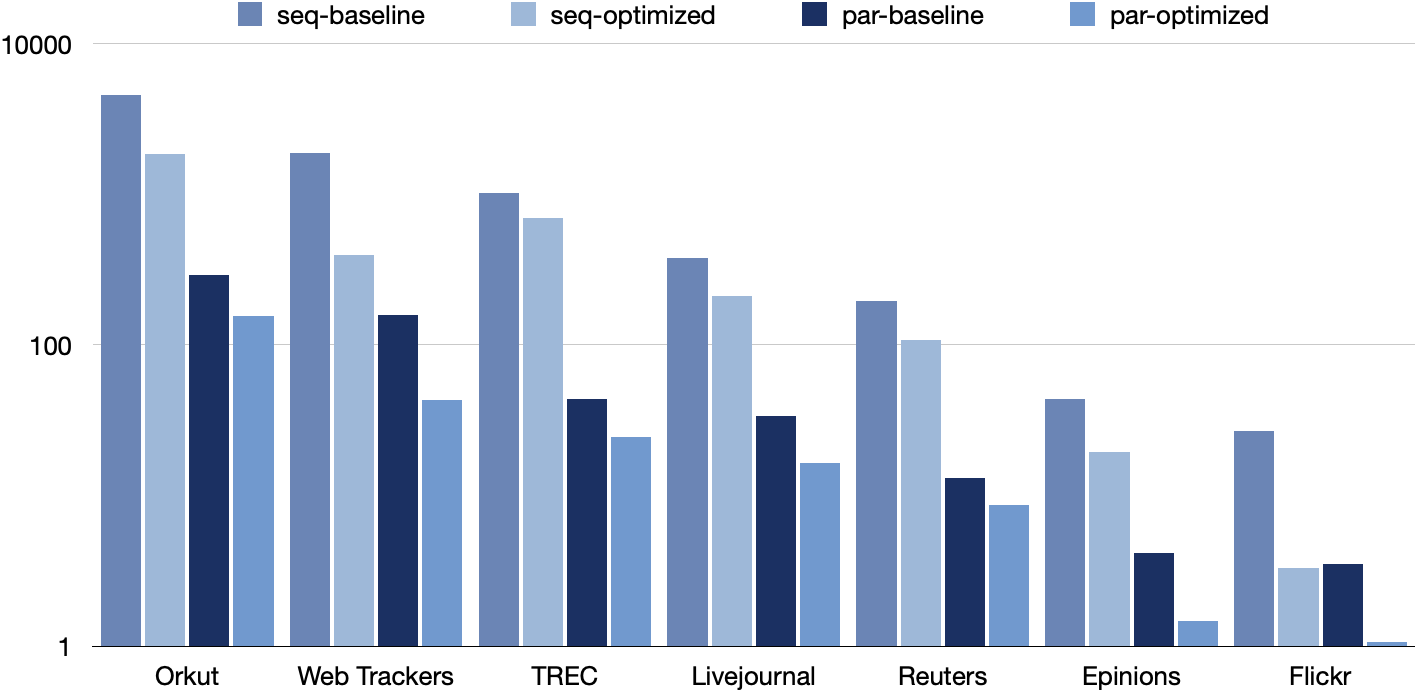
\includegraphics[width=7cm]{figures/log-runtime-comp.png} }}%
    \qquad
    \subfloat[\centering runtimes ]{{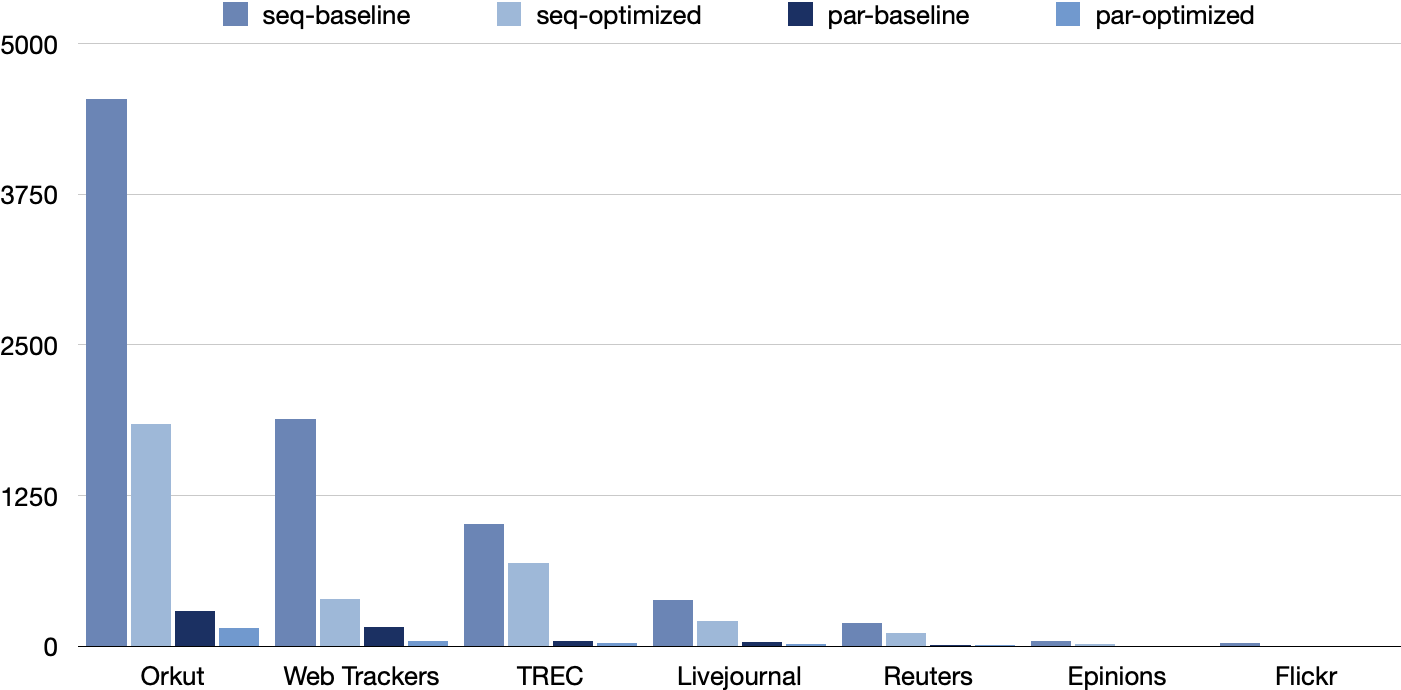
\includegraphics[width=7cm]{figures/linear-runtime-comp.png} }}%
    \caption{This figure comparatively shows the runtime (in seconds) of the 4 bi-core decomposition algorithms, \algname{seq-baseline}, \algname{seq-optimized}, \algname{par-baseline}, \algname{par-optimized}. Graph (a) is in log-scale while graph (b) is in linear-scale. \algname{par-optimized} consistently performs all 3 other algorithms.}%
    \label{fig:runtimes}%
\end{figure}

\myparagraph{Performances Comparison}

Figure \ref{fig:runtimes} shows the runtimes of the $4$ algorithms for graphs in Table \ref{tab:graphs}. The parallel algorithms are run with 30 threads. We do not run on 60 threads because the extra threads are hyperthreads and are not actual cores. Therefore, we observed that using 60 hyperthreads did not improve our running times.

\algname{par-baseline} and \algname{par-optimized} significantly outperforms \algname{seq-baseline} and \algname{seq-optimized}. While the parallel algorithms can process graphs with hundreds of millions of edges within several minutes, the sequential algorithms can take more than an hour to finish.

Running on 30 threads, \algname{par-optimized} attains 23--44x speedup over \algname{seq-baseline}, the sequential state of the art.

To compare against the parallel state of the art, also introduced by Liu \textit{et al.}, we note that they reported a runtime for 12 threads of 732 seconds for the Orkut graph. On the other hand, still running on 12 threads, \algname{par-optimized} attains a runtime of 253 seconds for the Orkut graph. Thus, our algorithm achieves a 2.9x speedup over Liu \textit{et al.}'s parallel algorithm, demonstrating the effectiveness of out introduced optimizations.

% \jessica{Generally when comparing to other people's work, it's better to be a bit delicate about it and give them as much benefit of doubt as possible. In 7.2, when discussing other implementations, I'd put in this kind of comment where we were not able to obtain their source code (this is nicer than saying that we weren't able to compile their source code), which is why we implement our own baselines to compare against. Then, in 7.2, you'd also say something like, we compare against their reported numbers in our analysis. I would not mention the kind of CPUs their using -- just say that they get x time on x cores, and for the same number of cores, we obtain x time. Also, don't mention that they only report concrete numbers for orkut; just write the comparison for orkut, and leave it at that.}

Figure \ref{fig:runtimes} also demonstrates the effectiveness of the peeling space pruning optimization we introduce. \algname{seq-optimized} consistently outperforms \algname{seq-baseline} by 2.1-2.8x. Similarly, \algname{par-optimized} is about 1.6-4.2x faster than \algname{par-baseline}. This demonstrates the effectiveness of the optimization technique across sequential and parallel setting. 

\begin{figure}%
    \centering
    \subfloat[\centering Speedup Ratios for Tested Graphs]{{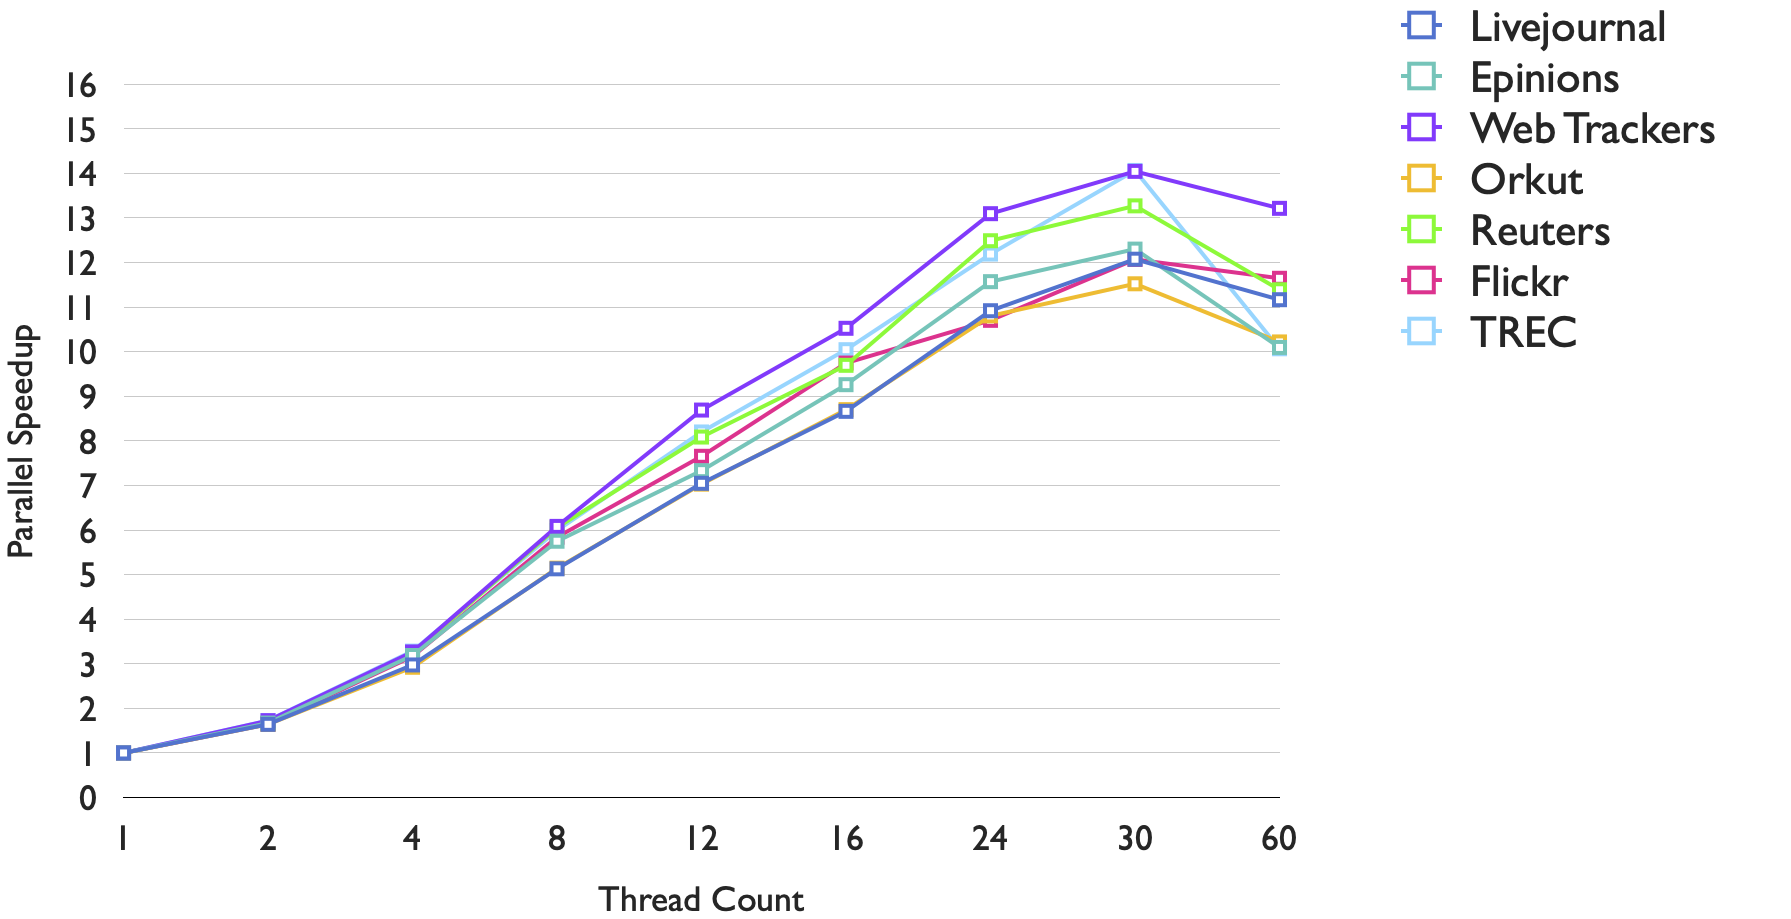
\includegraphics[width=7cm]{figures/speedup.png} }}%
    \qquad
    \subfloat[\centering Ratio of Runtimes Relative to Serial Time]{{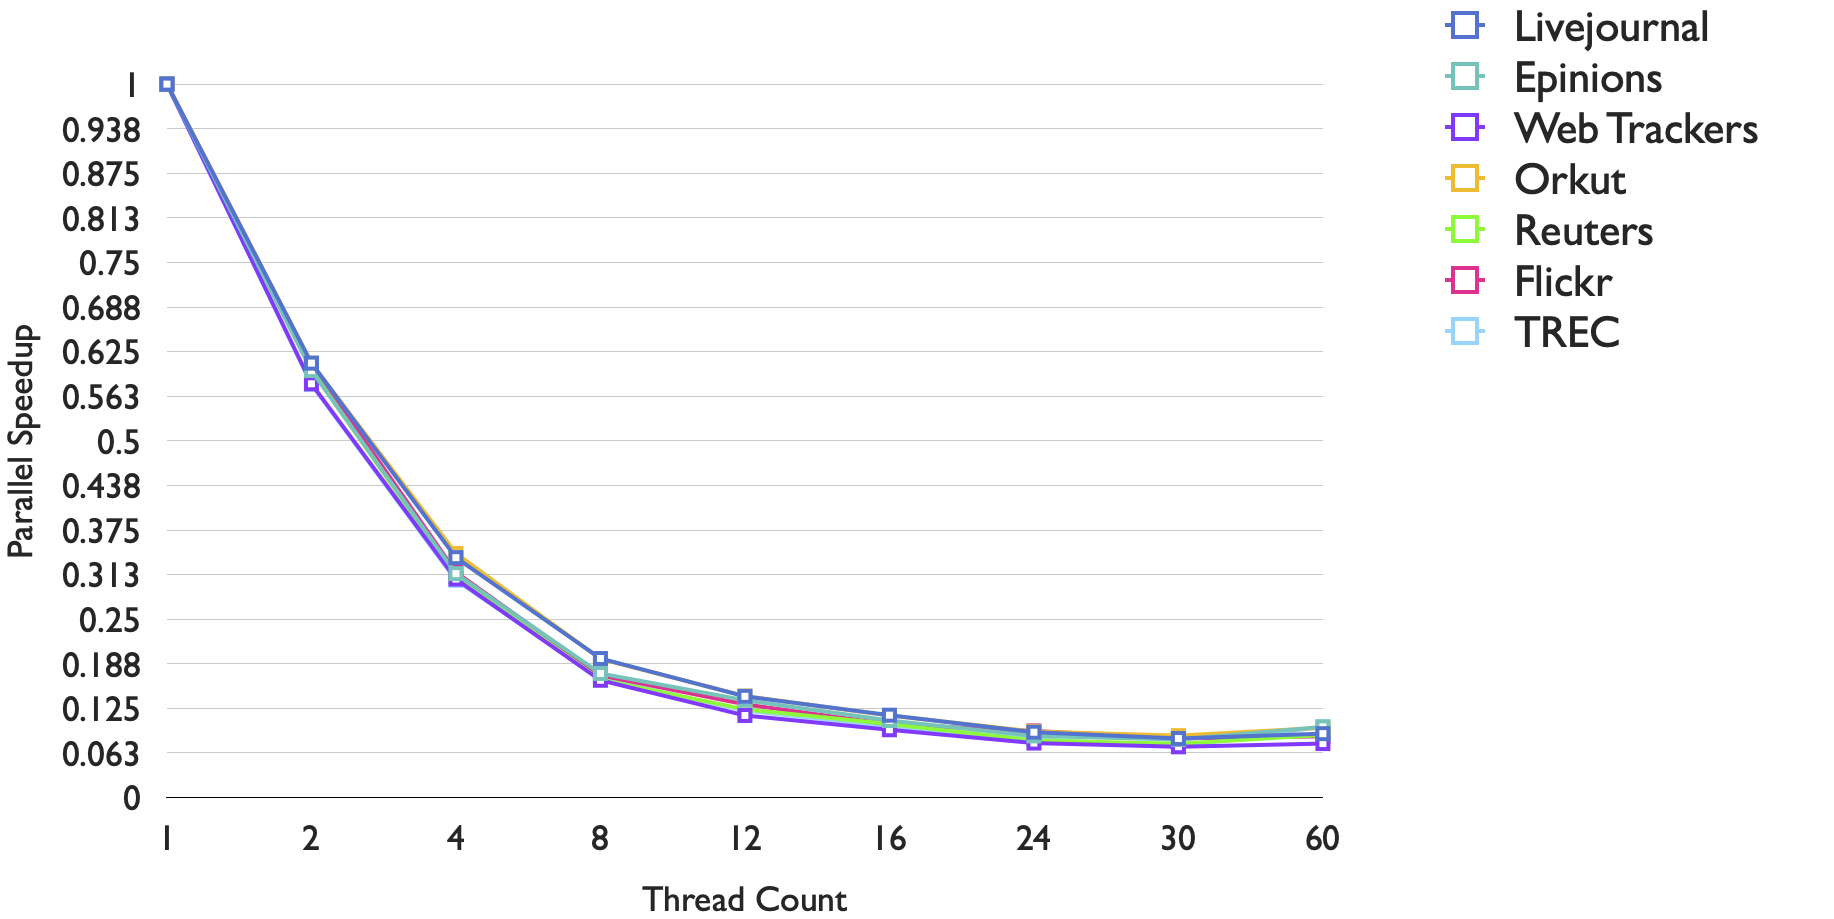
\includegraphics[width=7cm]{figures/runtime-ratio.png} }}%
    \caption{Graph (a) shows plots of the runtime of \algname{par-optimized} across different number of threads for various graphs. The plots show consistent speedups. Graph (b) shows the runtime ratios, which are the multiplicative inverses of the speedup numbers}%
    \label{fig:speedup}%
\end{figure}

\myparagraph{Analysis of Scalability}

As shown in Figure \ref{fig:speedup}, \algname{par-optimized} achieves a 11.5–14.1x self-relative speedup when running on 30 threads compared to 1 thread. The speedup plateaus at 60 threads. Increasing from 30 threads to 60 threads introduces virtual hyper-threads and not physical cores. So it is expected that there is no significant runtime improvement.

Further, Figure \ref{fig:speedup} demonstrates that the speedup achieved by \algname{par-optimized} is consistent across different graphs, showing that \algname{par-optimized} is scalable to graphs of sizes up to hundreds of millions of edges without noticeable deterioration in its parallel speedup. 

%\myparagraph{Analysis of $\rho$ vs runtime}

%\begin{figure}  
%\begin{center}  
%\includegraphics[width=0.8\columnwidth]{figures/rho-runtim%e.png}\caption{Rho value vs. Runtimes}\label{fig:rho}
%\end{center}  
%\end{figure}  

%The span of our algorithm is $\BigO{\rho \log(n)}$ \textit{w.h.p.} Theoretically, $\rho$ is bounded by $\BigO{\max(\text{dmax}_u,\text{dmax}_v)}=\BigO{n}$. Therefore, it is theoretically reasonable to assume that $\rho$ is the dominant term in the span. That is empirically true. For graphs given in Table \ref{tab:graphs}, the $\rho$ values are significantly larger than $\log_2(n)$ values. Thus, it is natural to assume there is an approximately linear correlation between the runtimes of \algname{par-optimized} and the $\rho$ values. Indeed, figure \ref{fig:rho} experimentally demonstrates a near-linear correlation between the $\rho$ values and the runtimes. This demonstrates that the bi-core peeling complexity we introduced is an important value in both theoretical and empirical evaluation of parallel bi-core decomposition algorithms.  

\subsection{Bi-core Index Construction}\label{sec:exp-index-cons}

\begin{figure}%
    \centering
    \subfloat[\centering Speedup Ratios for Tested Graphs]{{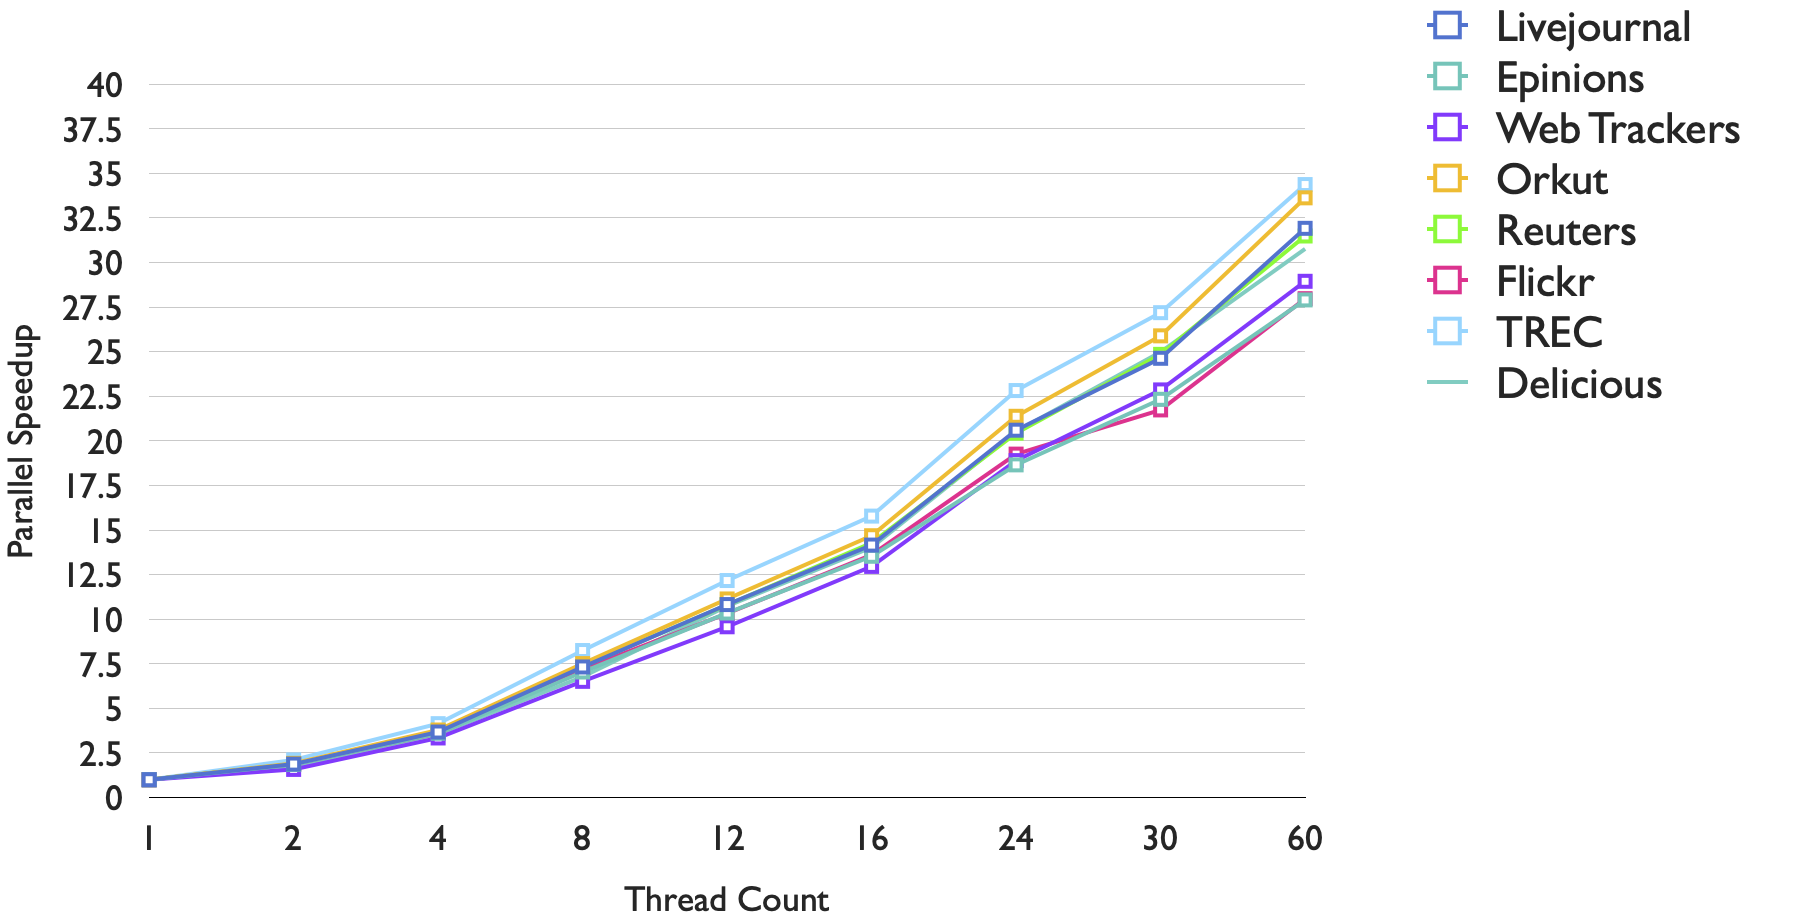
\includegraphics[width=7cm]{figures/speedup-cons.png} }}%
    \qquad
    \subfloat[\centering Ratio of runtimes relative to serial time]{{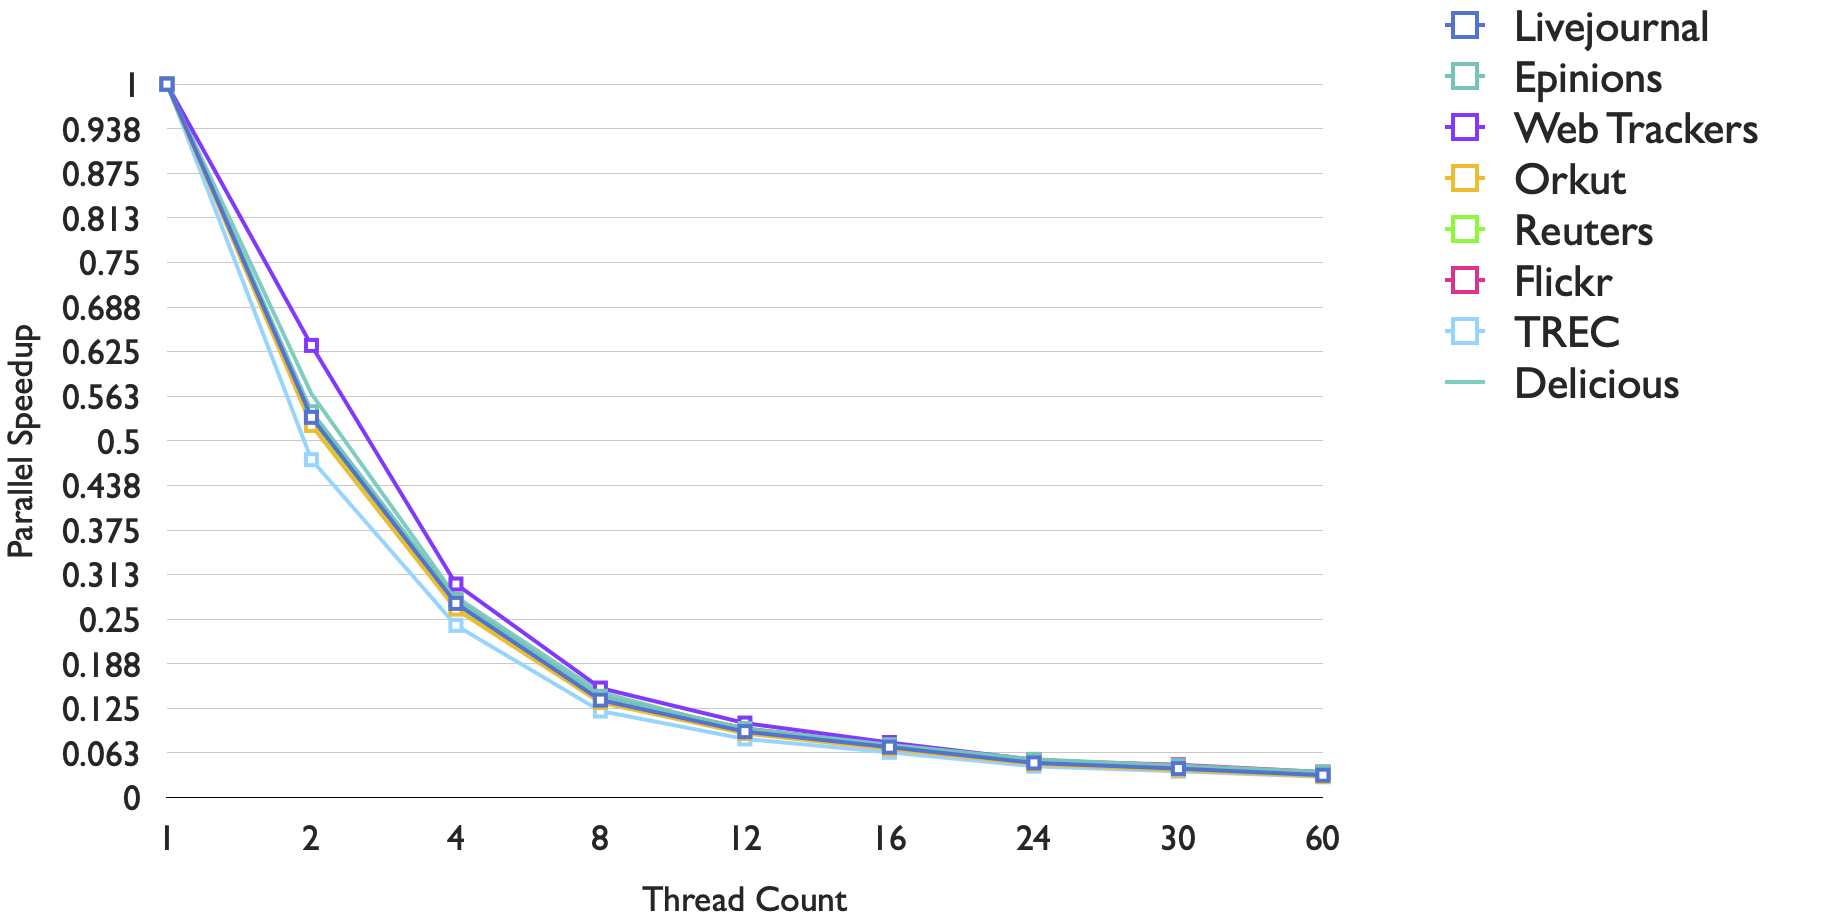
\includegraphics[width=7cm]{figures/runtime-ratio-cons.png} }}%
    \caption{Graph (a) shows plots of \algname{par-index}'s speedup over different number of threads used. Graph (b) shows the runtime ratios.}%
    \label{fig:speedup:c}%
\end{figure}

Now, we report the runtimes of the bi-core index construction algorithm, or \algname{par-index}. Using 30 threads, \algname{par-index} terminates for most graphs within several seconds. For example, when run on Orkut, a graph with 327 millions edges, with 30 threads, \algname{par-index} takes only 3.76 seconds to finish. This is $2.4\%$ of the runtime of \algname{par-optimized}. \algname{par-index} takes up similar percentage of time for other large graphs while taking up larger portion of time for smaller graphs. For example, on Flickr, \algname{par-index} is $10\%$ of \algname{par-optimized} in terms of runtime. This observation matches the theoretical prediction based on \algname{par-index}'s lower work complexity as compared to \algname{par-optimized}, which predicts that the runtime of \algname{par-optimized} grows faster than that of  \algname{par-index} as the number of edges increases.

\myparagraph{Analysis of Scalability}

Given its span of $\BigO{\log(n)}$, \algname{par-index} predictably has significant parallelism. Figure \ref{fig:speedup:c} demonstrates the parallel speedup of \algname{par-index} across different number of threads and different graphs used. Running on Delicious with 30 threads, \algname{par-index} achieves a near-linear self-relative speedup of 25.0x. A similar speedup number is achieved for all other graphs, as shown in Figure \ref{fig:speedup:c}. This demonstrates \algname{par-index} to be scalable to graphs of large sizes.

\subsection{Bi-core Index Query}\label{sec:exp-index-q}

\begin{figure}%
    \centering
    \subfloat[\centering Speedup ratios for tested graphs]{{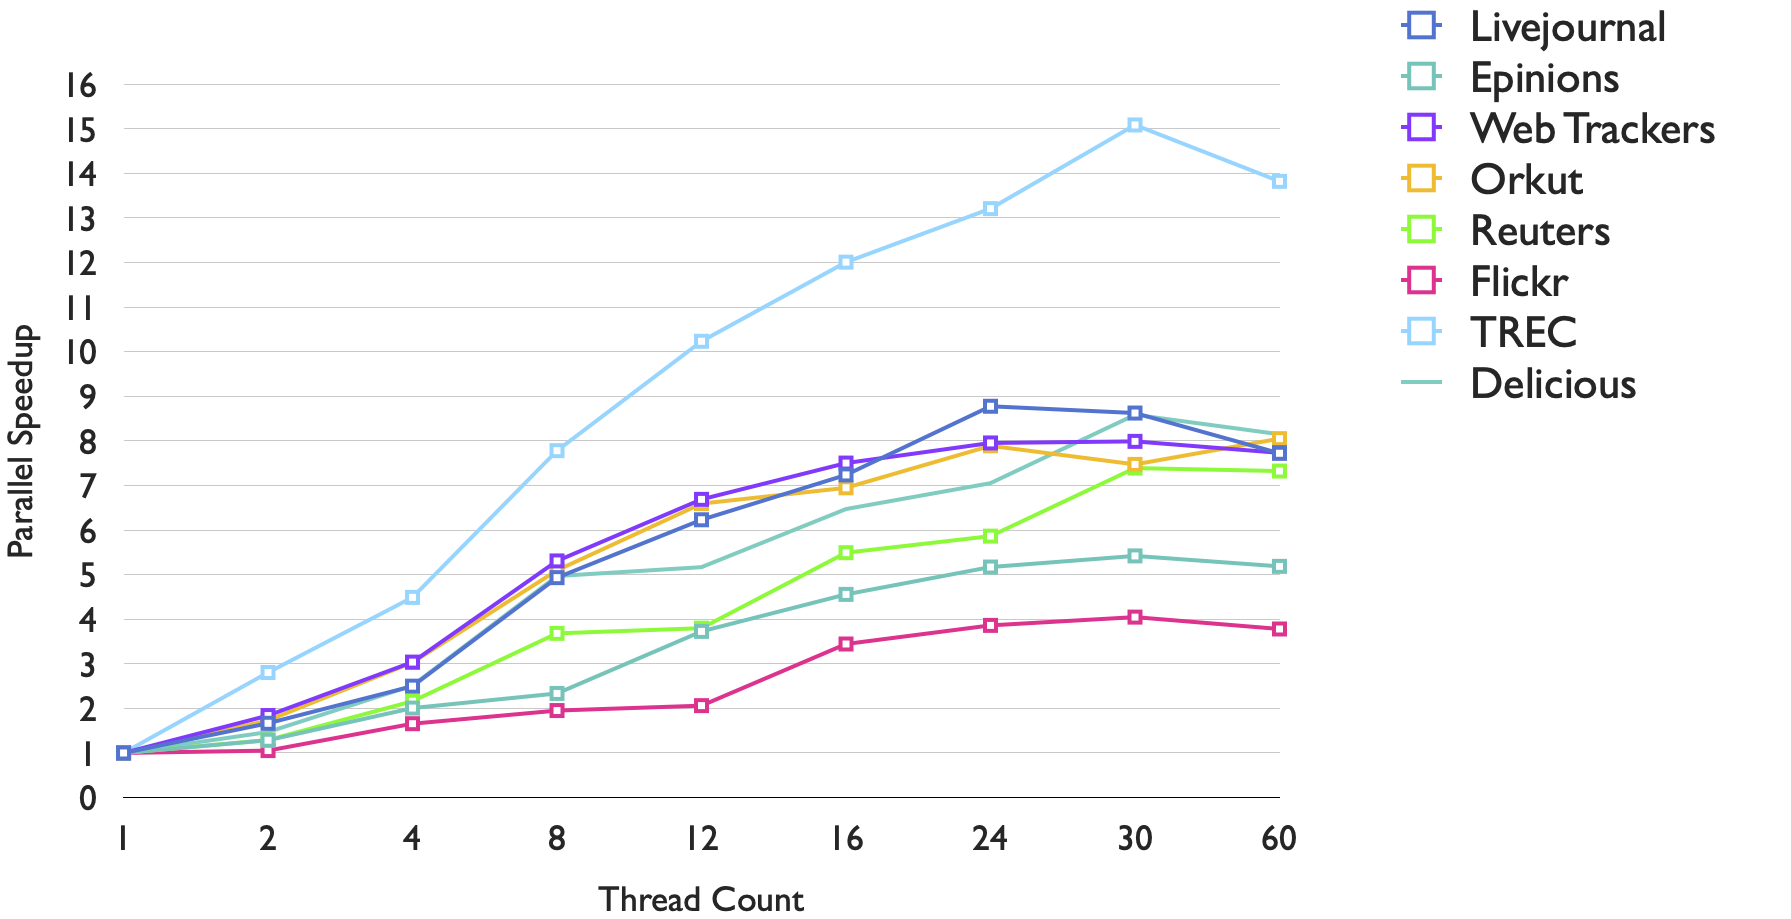
\includegraphics[width=7cm]{figures/speedup-q.png} }}%
    \qquad
    \subfloat[\centering Ratio of runtimes relative to serial time]{{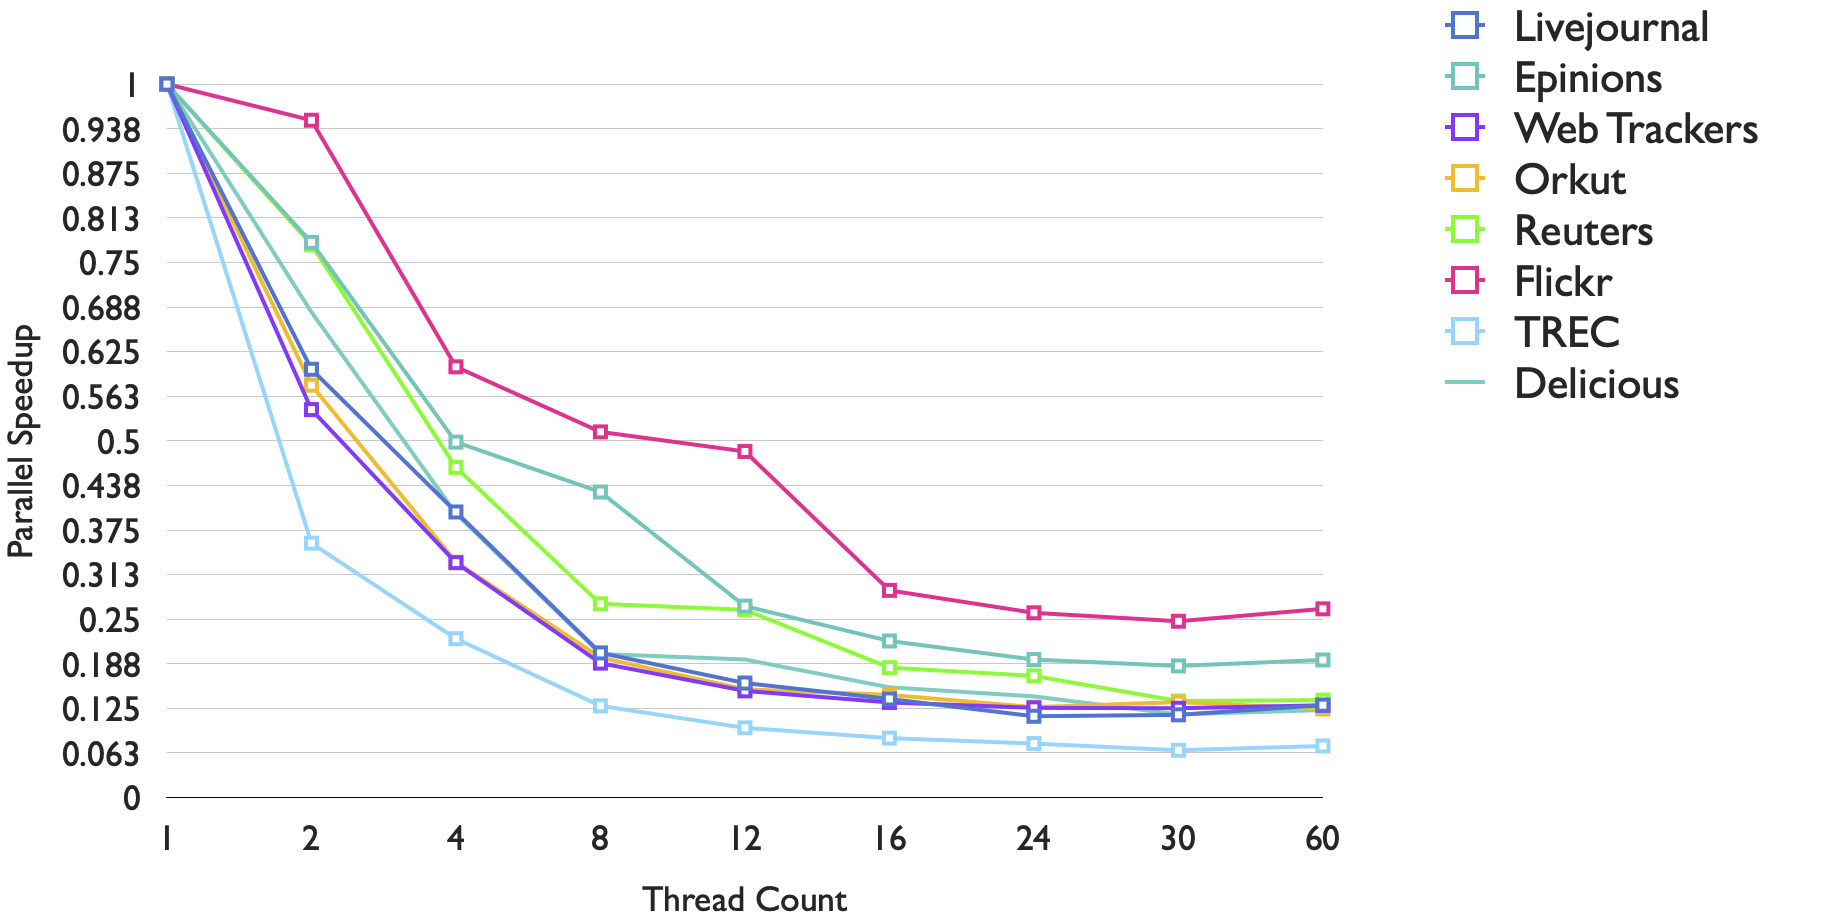
\includegraphics[width=7cm]{figures/runtime-ratio-q.png} }}%
    \caption{Graph (a) shows plots of \algname{par-query}'s speedup over different number of threads used. Graph (b) shows the runtime ratios.}%
    \label{fig:speedup:q}%
\end{figure}

In this section, we give the runtimes of our bi-core index query algorithm. Following the convention adopted by Liu \textit{et al.}, we report the runtime of completing 10 query calls with each query having $\alpha=10,\beta=10$. On the graph Delicious, Liu \textit{et al.} reported a runtime of 0.04 second. \algname{par-query}, running on a single thread, outperforms it, attaining a runtime of 0.0154 second. Our implementation achieves a 2.6x speedup. This proves that our optimization of storing the index structure in CSR format is effective (it potentially reduces the number of cache misses). Using 30 threads, \algname{par-query} achieves a runtime 0.0018 second, which is a 22.3x speedup over the Liu \textit{et al.}'s sequential query algorithm. 

\myparagraph{Analysis of Scalability}

Figure \ref{fig:speedup:q} demonstrates the tangible self-relative speedups achieved by \algname{par-query}. It achieves up to 15.1x self-relative speedup using 30 threads as compared to 1 thread. The speedup achieved is mostly consistent across different graphs, but has higher volatility when compared to the \algname{par-optimized} or \algname{par-index}. This is expected due to the low runtime of the query algorithm as well as its strong dependence on cache efficiency, with parallel copy of contagious array being its only time-consuming operation. 
